% The BLAKE2 mixing function G [RFC 7693, §3.1] on words a, b, c, d of the work vector, with
% message words x and y. Additions are modulo 2^w; the rotations (R1, R2, R3, R4) are
% (32, 24, 16, 63) for BLAKE2b and (16, 12, 8, 7) for BLAKE2s.
% Original drawing for the Hash library.
\documentclass[tikz,border=6pt]{standalone}
\usepackage[T1]{fontenc}
\usepackage{lmodern}
\usepackage{amssymb}
% Shared style for the Hash diagrams.
% Palette: Okabe–Ito (colour-blind safe). Every diagram is drawn on an opaque white card so it
% stays legible on dark page themes.
\usetikzlibrary{arrows.meta,positioning,calc,fit,backgrounds}
\definecolor{hsblue}{HTML}{0072B2}
\definecolor{hsorange}{HTML}{E69F00}
\definecolor{hsgreen}{HTML}{009E73}
\definecolor{hsvermilion}{HTML}{D55E00}
\definecolor{hspurple}{HTML}{CC79A7}
\definecolor{hsink}{HTML}{1F2933}
\tikzset{
  >={Stealth[length=2.2mm]},
  every node/.style={font=\sffamily\small, text=hsink},
  wire/.style={draw=hsink, line width=0.6pt, ->},
  reg/.style={draw=hsink, line width=0.6pt, fill=hsblue!12, minimum width=9mm, minimum height=7mm},
  fn/.style={draw=hsink, line width=0.6pt, fill=hsorange!25, rounded corners=2pt, minimum width=10mm, minimum height=6mm},
  input/.style={draw=hsink, line width=0.6pt, fill=hsgreen!20, minimum width=9mm, minimum height=6mm},
  add/.style={circle, draw=hsink, line width=0.6pt, fill=white, inner sep=0pt, minimum size=5mm, font=\sffamily\bfseries},
  card/.style={fill=white, rounded corners=4pt},
}

\begin{document}
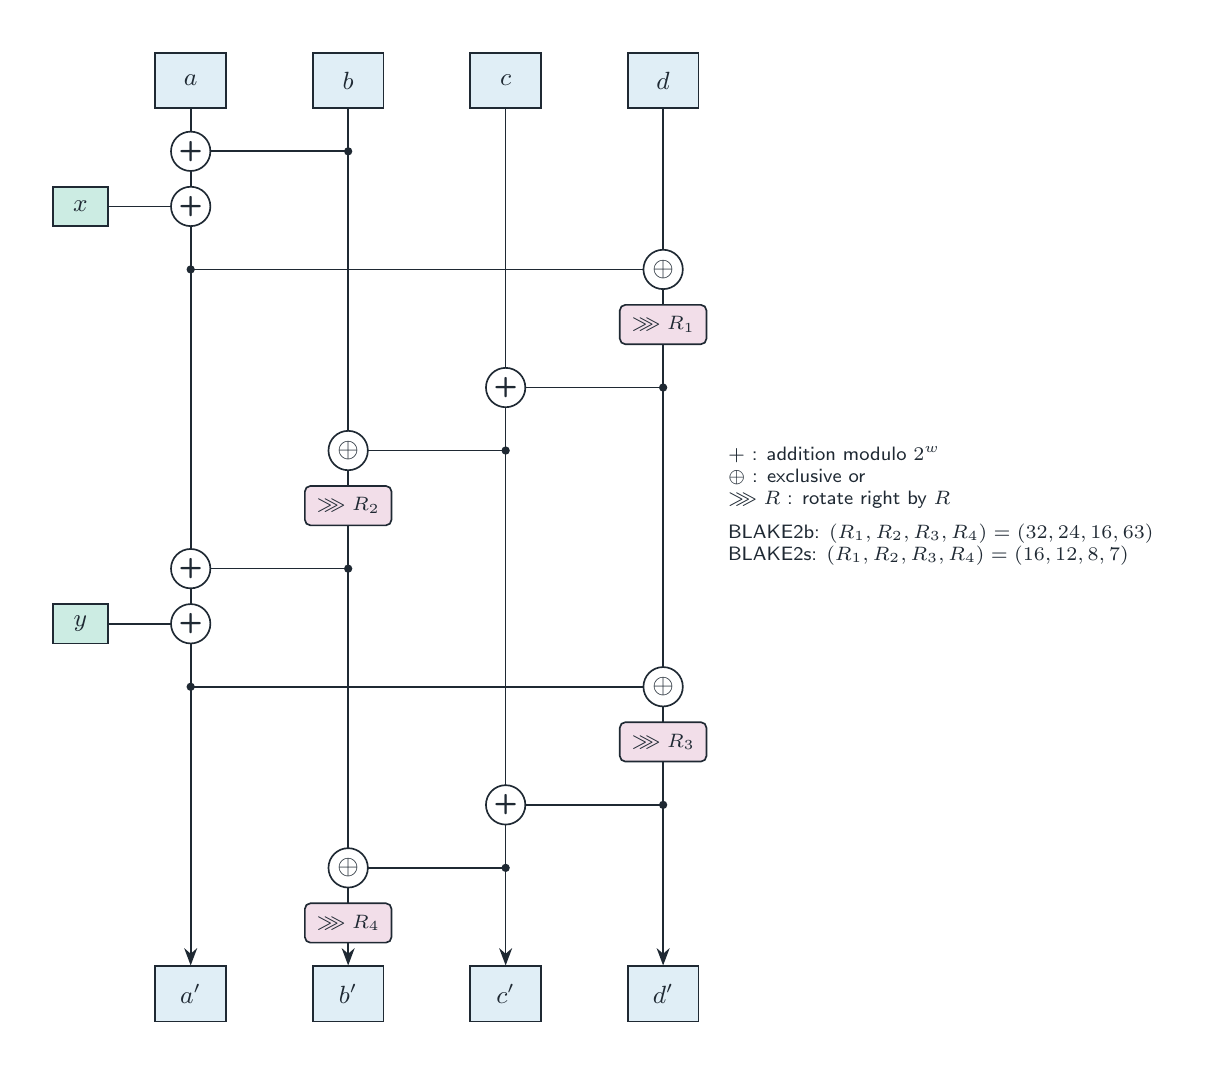
\begin{tikzpicture}[rot/.style={fn, fill=hspurple!25, minimum width=11mm, minimum height=5mm,
    font=\sffamily\scriptsize}, dot/.style={circle, fill=hsink, inner sep=0pt, minimum size=3pt}]
  \def\xa{0}\def\xb{2.0}\def\xc{4.0}\def\xd{6.0}
  \foreach \v/\x in {a/\xa, b/\xb, c/\xc, d/\xd} {
    \node[reg] (in\v) at (\x, 0) {$\v$};
    \node[reg] (out\v) at (\x, -11.6) {$\v'$};
    \draw[wire] (in\v) -- (out\v);
  }
  % op: target column x, source column x, y, symbol.
  \newcommand{\op}[4]{%
    \node[dot] at (#2, #3) {};
    \draw[wire] (#2, #3) -- (#1, #3);
    \node[add] at (#1, #3) {#4};}
  \newcommand{\rot}[3]{\node[rot] at (#1, #2) {$\ggg #3$};}
  \newcommand{\msg}[3]{%
    \node[input, minimum width=7mm, minimum height=5mm] (m#3) at (-1.4, #2) {$#3$};
    \draw[wire] (m#3) -- (#1, #2);
    \node[add] at (#1, #2) {+};}
  \op{\xa}{\xb}{-0.9}{+}  \msg{\xa}{-1.6}{x}
  \op{\xd}{\xa}{-2.4}{$\oplus$} \rot{\xd}{-3.1}{R_1}
  \op{\xc}{\xd}{-3.9}{+}
  \op{\xb}{\xc}{-4.7}{$\oplus$} \rot{\xb}{-5.4}{R_2}
  \op{\xa}{\xb}{-6.2}{+}  \msg{\xa}{-6.9}{y}
  \op{\xd}{\xa}{-7.7}{$\oplus$} \rot{\xd}{-8.4}{R_3}
  \op{\xc}{\xd}{-9.2}{+}
  \op{\xb}{\xc}{-10.0}{$\oplus$} \rot{\xb}{-10.7}{R_4}
  \node[anchor=west, font=\sffamily\scriptsize, align=left] at (6.7,-5.4)
    {$+$ : addition modulo $2^w$\\ $\oplus$ : exclusive or\\ $\ggg R$ : rotate right by $R$\\[4pt]
     BLAKE2b: $(R_1, R_2, R_3, R_4) = (32, 24, 16, 63)$\\
     BLAKE2s: $(R_1, R_2, R_3, R_4) = (16, 12, 8, 7)$};
  \begin{scope}[on background layer]
    \coordinate (e1) at (-2.0,-12.2);
    \coordinate (e2) at (12.6,0.6);
    \node[card, fit=(e1)(e2), inner sep=2pt] {};
  \end{scope}
\end{tikzpicture}
\end{document}
